\pagebreak
\section{The genetic algorithm}

\subsection{Description of genetic algorithms}
Genetic algorithms are based on the idea of evolution, that the most suited individuals tend to live longer and reproduce. A population is simulated in an artificial world using a combination of reproduction, gene crossover and mutation, with a given goal to achieve. The population consists of individuals, which by simplification has one chromosome each, containing one or more genes. During each generation, reproduction is performed to create new individuals, called children.\\
\\
Due to the need to simulate the population and evaluate individuals, often multiple times, GA's are not well suited for all kind of problems. When there exists an analytical solution it may be better to use that.\\* %% Because of?
However if the problem can be simulated both problems without analytical solutions and problem with complicated analytical solution can be handled by GA's, although it is never guaranteed to give an optimal solution.\\
%% Variations / Generational / Steady-state
There are different ways to implement genetic algorithms, with variations in how each step is performed. This yields many different versions of genetic algorithms. First there are two different kinds of GA's, steady-state and generational. Steady-state maintains and alters one population by replacing its individuals through reproduction, while generational replaces an old population with a new one.
Figure~\ref{GeneticFlowChart1} shows a flowchart of a genetic algorithm.
\begin{figure}[!h]
	\centering
	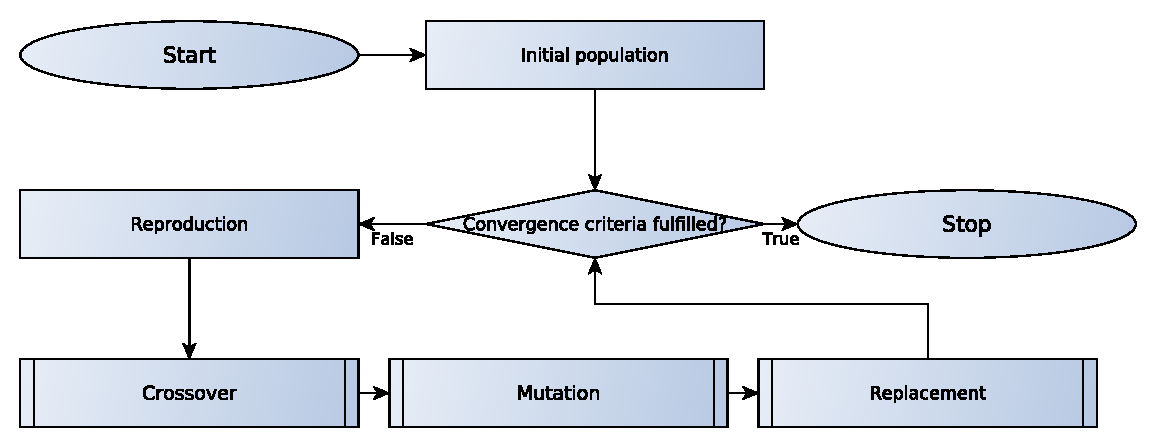
\includegraphics[width=\textwidth]{chapter_4_methods/GeneticFlowChart-Generic}
  	\caption[Flowchart of a genetic algorithm]
  	{Flowchart of a genetic algorithm}
	\label{GeneticFlowChart1}
\end{figure}
%% Initial population
\\At first an initial population has to be obtained, either by an existing set of solutions or by creation.\\*
%% Evaluation / Fitness function
To determine a solution the individuals has to be evaluated and compared to each other. For that a fitness function is used, which is to calculate a score for an individual depending on how well it fulfils the goal.\\
%% Reproduction
To widen the search for solutions evolution is performed by a reproduction step, during which two individuals are selected and used to create two new individuals. The new individuals are created first by crossover and then subject to mutation.\\
%% Selection (parents)
For selection, there are different methods but five of them are Fitness Proportionate Selection, Random Selection, Fit-Fit, Elite selection and tournament selection.\\
In Fitness Proportionate Selection, of which Roulette Selection is one example, the probability of choosing a more fit individual is higher than to select a less fit individual.\\
In Random Selection, the probability to be selected is equal for all individuals. \\
With Fit-fit, at each step the two most fit individuals are selected. In the next step the next two most fit are selected.\\
In Elite selection the best individual is chosen. This selection procedure should be used in combination with another selection method.\\
Tournament selection chooses a number of individuals stochastically, and then take the best of them.\\
\\
%% Crossover
For Crossover there are different methods, a few of those are n-point shuffle crossover, uniform crossover and variable crossover.\\
\\
%% Mutation
\\Mutation is important in GA's since it makes sure that all the search space can be reached, even if the initial population did not cover all of it. It can be implemented as 'bit-flip', if the gene is binary encoded, where a 0 is changed to 1 and 1 to 0.\\
\\
%% Replacement
When breeding has been completed, in order to not increase the population size, a replacement has to be performed. For this there are several methods, such as Weak Parent, Both Parents, Weakest Individual and Random.\\
In Weak Parent, a weaker parent is replaced by a stronger child.\\
In Both Parents, the children replaces the parents.\\
In Weakest Individual, the children replaces the two weakest individuals in the population, if the children are fitter.\\
In Random, the children replaces random individuals in the population.\\
\\
%% Termination
To make sure the algorithm ends at some point, a termination condition has to be used, for instance a maximum number of generations, a limit in fitness sum, a median fitness, best individual or worst individual.\\
With Fitness sum, the algorithm will terminate when the sum of the fitness for the population is less than or equal to a specified value.\\
With Median fitness, a range for the fitness is specified.\\
With best individual, the algorithm will terminate when the minimum fitness drops below a convergence value and thereby guarantee at least one good solution while saving time.\\
With Worst Individual, the algorithm will terminate when all individuals in the population has a fitness value lower than the convergence value.\\
\\
%% Encoding
To adapt genes to computers, an encoding has to be used.  According to literature \cite{GAHandbook1} binary encoding is the fastest encoding, where each gene is encoded as 0 and 1, but there are also integer encoding and string encoding.\\
%%%% Development process of the genetic algorithm
\subsection{Development process of the genetic algorithm}
The first idea to use  was to use an existing framework for Genetic Algorithms, such as LibGA or GAUL, to save time on programming. Due to the implementation of the libraries, for this application it was determined to be faster to write a new implementation.\\
\\After reading parts of the source code of existing libraries and Johan Thunberg's Boolean Control software \cite{paper1} for ideas, a first attempt to a program was written. The first version was a boolean control network, where feasible solutions were generated by using a random function to generate numbers between 0 and 4 to indicate if the pursuer were to move left, right, up, down or stand still. For each pursuer, an integer based encoding was used, which was easy to implement and debug compared to binary encoding. Each digit in the gene is called an allele, following the notation from \cite{GA-ai}. It was thereafter extended to a generational GA instead of steady-state, because of easier implementation and a more clear termination condition in number of generations. \\
%% Fitness
At first a simple fitness function with two variables was used \eqref{fitness1}, S4 which is the number of nodes in state 4 and \textbf{step} which is the total number of steps taken to minimize S4.
\begin{equation}\label{fitness1} (1+S4+steps) \end{equation}
A change of selection procedure, see next paragraph, made it necessary to switch to a function which was to be maximized \eqref{fitness2},  where the numerator was used to scale the fitness value closer to positive integer values.
\begin{equation}\label{fitness2} \frac{1000}{(1+S4+steps)} \end{equation}
The final version of the fitness function was a simplified version of \eqref{fitness2}. By using the total number of nodes, called Nodes,  and the maximum allowed steps, called MaxSteps, the fitness function was limited to positive integer values, which should be easier for a computer to calculate.
\begin{equation} \label{fitness3}Nodes-S4+MaxSteps-steps \end{equation}
%% Selection
\\For selection, Random, Tournament  and Fitness Proportionate Selection were considered, all three in combination with elite selection to avoid loosing the best solution found. Random selection is the easiest to implement and was first used to create a working GA, but it was replaced with Tournament selection as it gives a more fit individual an advantage. In the final version a Fitness Proportionate Selection was used, which gives more fit solutions an even greater advantage and thereby helps the population converge even faster. Elite selection was used to keep track of the two best solution each generation.\\
%% Crossover
\\To make the crossover operation easy to implement, a version of n-point crossover was used. One path from each pursuer was used alternating from each parent.\\
%% Mutation
\\Due to the integer encoding, and node network representation, 'bit-flip' was not easily implemented. Instead a gene is selected by a random function, and thereafter a random allele is chosen to be replaced. When an allele is replaced all following alleles are generated again to make sure the path generated is feasible.
%% Replacement
\\To make sure the overall fitness of the population increased, a weak parent replacement was used.\\
%% Parameters
\\At first a population size of 400 was used, which was what worked best after 10 trial runs at 5x5, in combination with a limit of 100 generations and 200 steps/alleles. Mutation frequency was set to 5\% after testing different values, which is more than the often used value in literature \cite{GAHandbook2} of 1-2\%, but still not very large. The parameters varied, and due to the increasing computation time with increasing population size a relatively small population of a maximum of 2000 individuals was used, in combination with a high mutation rate of 75\% and a maximum of 800 generations. This was in order to cover a large search space when working with environments larger than 5x5 nodes, without having an population size of over 4.000 which at some attempts took over 10 minutes for a single generation. The final version of the program had a more dynamic population size and step length, see next subsection.

\subsection{The genetic algorithm of our problem}
The final version of the genetic algorithm had a maximum population of 2000 individuals and 600 steps\footnote{depending on the size of the environment the maximum number of steps was set between 50 and 600 }, but during initialization the population size and step length was limited to a lower value if possible. This was done by creating an initial population of 400 individuals, evaluating each and see if any solution clears the environment. If it does, the maximum step length is limited to the number of steps used, and the population is incremented by 100 individuals to increase the probability of having a diversity in the population.
\begin{figure}[!h]
	\centering
	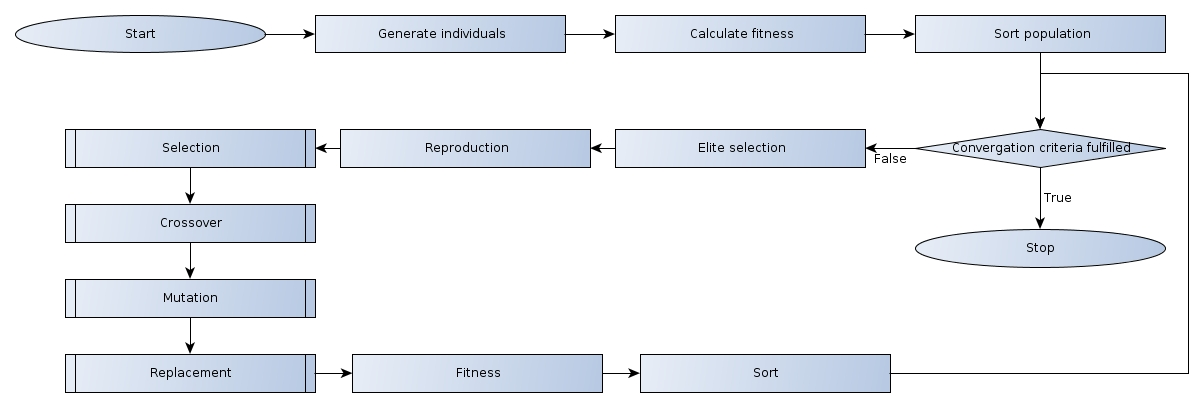
\includegraphics[width=\textwidth]{chapter_4_methods/GeneticFlowChart-Algorithm}
	\caption[Flowchart of the implemented genetic algorithm]
	{Flowchart of the implemented genetic algorithm}
\end{figure}
%% Initial population
\\As written in the previous subsection the initial population was generated by a random function, which gave each pursuer a sequence of alleles that represented each step.
%% Fitness 
Each individual was evaluated using \eqref{fitness3}, and sorted by fitness in decreasing order, which facilitated selection.
%% Breeding
The two individuals with the best fitness value was added to the new population, and thereafter the selection process selected individuals for breeding. Fitness proportionate selection was used, in which the sum of the fitness value was calculated and a random number between 0 and the sum was generated. The fitness was thereafter added for each individual until that number was reached, and that individual was selected. This was repeated to select a second parent. The crossover was copying genes alternating between each parent, so that two different children were created. A mutation step was performed with 75\% probability, where an allele from one of the gene was replaced as described in the previous subsection. Finally the best individuals of the parents and children was  placed in the new population, and the step is repeated until a new population of the same size as the previous was created.
%% Termination
As a termination criteria the fitness score of up to 99\%\footnote{Values between 50\% and 99\% was used} of the population was compared. If the individuals had completely cleared the environment and had an equal fitness score, the algorithm was terminated. As 99\% is a very high convergence criteria, it was only used for small environments to avoid premature termination. As a second termination criteria the maximum number of generations was set to 800, to make sure the algorithm would terminate even if no solution was found.
\subsection{Our implementation of the genetic algorithm}
The algorithm was implemented using C. Every time a random value was to be obtained \begin{verbatim} ((int)((double)rand() / ((double)RAND_MAX + 1)*SCALE_FACTOR)); \end{verbatim} was used, which generates a number in the range [0,SCALE\_FACTOR). As a random seed number \begin{verbatim} srand(time(0))\end{verbatim} was used. No alternative random functions were evaluated.\\
For sorting the population, quicksort was used \cite{quicksort}.\\